% Options for packages loaded elsewhere
\PassOptionsToPackage{unicode}{hyperref}
\PassOptionsToPackage{hyphens}{url}
%
\documentclass[
]{article}
\usepackage{amsmath,amssymb}
\usepackage{iftex}
\ifPDFTeX
  \usepackage[T1]{fontenc}
  \usepackage[utf8]{inputenc}
  \usepackage{textcomp} % provide euro and other symbols
\else % if luatex or xetex
  \usepackage{unicode-math} % this also loads fontspec
  \defaultfontfeatures{Scale=MatchLowercase}
  \defaultfontfeatures[\rmfamily]{Ligatures=TeX,Scale=1}
\fi
\usepackage{lmodern}
\ifPDFTeX\else
  % xetex/luatex font selection
\fi
% Use upquote if available, for straight quotes in verbatim environments
\IfFileExists{upquote.sty}{\usepackage{upquote}}{}
\IfFileExists{microtype.sty}{% use microtype if available
  \usepackage[]{microtype}
  \UseMicrotypeSet[protrusion]{basicmath} % disable protrusion for tt fonts
}{}
\makeatletter
\@ifundefined{KOMAClassName}{% if non-KOMA class
  \IfFileExists{parskip.sty}{%
    \usepackage{parskip}
  }{% else
    \setlength{\parindent}{0pt}
    \setlength{\parskip}{6pt plus 2pt minus 1pt}}
}{% if KOMA class
  \KOMAoptions{parskip=half}}
\makeatother
\usepackage{xcolor}
\usepackage[margin=1in]{geometry}
\usepackage{color}
\usepackage{fancyvrb}
\newcommand{\VerbBar}{|}
\newcommand{\VERB}{\Verb[commandchars=\\\{\}]}
\DefineVerbatimEnvironment{Highlighting}{Verbatim}{commandchars=\\\{\}}
% Add ',fontsize=\small' for more characters per line
\usepackage{framed}
\definecolor{shadecolor}{RGB}{248,248,248}
\newenvironment{Shaded}{\begin{snugshade}}{\end{snugshade}}
\newcommand{\AlertTok}[1]{\textcolor[rgb]{0.94,0.16,0.16}{#1}}
\newcommand{\AnnotationTok}[1]{\textcolor[rgb]{0.56,0.35,0.01}{\textbf{\textit{#1}}}}
\newcommand{\AttributeTok}[1]{\textcolor[rgb]{0.13,0.29,0.53}{#1}}
\newcommand{\BaseNTok}[1]{\textcolor[rgb]{0.00,0.00,0.81}{#1}}
\newcommand{\BuiltInTok}[1]{#1}
\newcommand{\CharTok}[1]{\textcolor[rgb]{0.31,0.60,0.02}{#1}}
\newcommand{\CommentTok}[1]{\textcolor[rgb]{0.56,0.35,0.01}{\textit{#1}}}
\newcommand{\CommentVarTok}[1]{\textcolor[rgb]{0.56,0.35,0.01}{\textbf{\textit{#1}}}}
\newcommand{\ConstantTok}[1]{\textcolor[rgb]{0.56,0.35,0.01}{#1}}
\newcommand{\ControlFlowTok}[1]{\textcolor[rgb]{0.13,0.29,0.53}{\textbf{#1}}}
\newcommand{\DataTypeTok}[1]{\textcolor[rgb]{0.13,0.29,0.53}{#1}}
\newcommand{\DecValTok}[1]{\textcolor[rgb]{0.00,0.00,0.81}{#1}}
\newcommand{\DocumentationTok}[1]{\textcolor[rgb]{0.56,0.35,0.01}{\textbf{\textit{#1}}}}
\newcommand{\ErrorTok}[1]{\textcolor[rgb]{0.64,0.00,0.00}{\textbf{#1}}}
\newcommand{\ExtensionTok}[1]{#1}
\newcommand{\FloatTok}[1]{\textcolor[rgb]{0.00,0.00,0.81}{#1}}
\newcommand{\FunctionTok}[1]{\textcolor[rgb]{0.13,0.29,0.53}{\textbf{#1}}}
\newcommand{\ImportTok}[1]{#1}
\newcommand{\InformationTok}[1]{\textcolor[rgb]{0.56,0.35,0.01}{\textbf{\textit{#1}}}}
\newcommand{\KeywordTok}[1]{\textcolor[rgb]{0.13,0.29,0.53}{\textbf{#1}}}
\newcommand{\NormalTok}[1]{#1}
\newcommand{\OperatorTok}[1]{\textcolor[rgb]{0.81,0.36,0.00}{\textbf{#1}}}
\newcommand{\OtherTok}[1]{\textcolor[rgb]{0.56,0.35,0.01}{#1}}
\newcommand{\PreprocessorTok}[1]{\textcolor[rgb]{0.56,0.35,0.01}{\textit{#1}}}
\newcommand{\RegionMarkerTok}[1]{#1}
\newcommand{\SpecialCharTok}[1]{\textcolor[rgb]{0.81,0.36,0.00}{\textbf{#1}}}
\newcommand{\SpecialStringTok}[1]{\textcolor[rgb]{0.31,0.60,0.02}{#1}}
\newcommand{\StringTok}[1]{\textcolor[rgb]{0.31,0.60,0.02}{#1}}
\newcommand{\VariableTok}[1]{\textcolor[rgb]{0.00,0.00,0.00}{#1}}
\newcommand{\VerbatimStringTok}[1]{\textcolor[rgb]{0.31,0.60,0.02}{#1}}
\newcommand{\WarningTok}[1]{\textcolor[rgb]{0.56,0.35,0.01}{\textbf{\textit{#1}}}}
\usepackage{graphicx}
\makeatletter
\def\maxwidth{\ifdim\Gin@nat@width>\linewidth\linewidth\else\Gin@nat@width\fi}
\def\maxheight{\ifdim\Gin@nat@height>\textheight\textheight\else\Gin@nat@height\fi}
\makeatother
% Scale images if necessary, so that they will not overflow the page
% margins by default, and it is still possible to overwrite the defaults
% using explicit options in \includegraphics[width, height, ...]{}
\setkeys{Gin}{width=\maxwidth,height=\maxheight,keepaspectratio}
% Set default figure placement to htbp
\makeatletter
\def\fps@figure{htbp}
\makeatother
\setlength{\emergencystretch}{3em} % prevent overfull lines
\providecommand{\tightlist}{%
  \setlength{\itemsep}{0pt}\setlength{\parskip}{0pt}}
\setcounter{secnumdepth}{-\maxdimen} % remove section numbering
\usepackage{fvextra}
\DefineVerbatimEnvironment{Highlighting}{Verbatim}{breaklines, commandchars=\\\{\}}
\usepackage{fvextra}
\ifLuaTeX
  \usepackage{selnolig}  % disable illegal ligatures
\fi
\IfFileExists{bookmark.sty}{\usepackage{bookmark}}{\usepackage{hyperref}}
\IfFileExists{xurl.sty}{\usepackage{xurl}}{} % add URL line breaks if available
\urlstyle{same}
\hypersetup{
  pdftitle={Problemas Propuesto Regresión Multinomial},
  pdfauthor={Francisco Javier Mercader Martínez},
  hidelinks,
  pdfcreator={LaTeX via pandoc}}

\title{Problemas Propuesto Regresión Multinomial}
\author{Francisco Javier Mercader Martínez}
\date{}

\begin{document}
\maketitle

\hypertarget{problema-1}{%
\section{Problema 1}\label{problema-1}}

El dichero \textbf{iris} de R, contiene los datos correspondientes de
los pétalos y sépalos de tres variedades de flor de iris (setosa,
virginica y versicolor).

Se desea realizar un análisis de Regresión Multinomial con el fin de
predecir la variedad de la flor en función de las magnitudes de sus
pétalos y sépalos. Se pide:

\begin{enumerate}
\def\labelenumi{\arabic{enumi})}
\tightlist
\item
  Recuperar los datos y realizar un estudio descriptivo previo
  atendiendo a nuestro objetivo.
\end{enumerate}

\begin{Shaded}
\begin{Highlighting}[]
\NormalTok{iris }\OtherTok{\textless{}{-}}\NormalTok{ iris}
\FunctionTok{summary}\NormalTok{(iris)}
\end{Highlighting}
\end{Shaded}

\begin{verbatim}
##   Sepal.Length    Sepal.Width     Petal.Length    Petal.Width   
##  Min.   :4.300   Min.   :2.000   Min.   :1.000   Min.   :0.100  
##  1st Qu.:5.100   1st Qu.:2.800   1st Qu.:1.600   1st Qu.:0.300  
##  Median :5.800   Median :3.000   Median :4.350   Median :1.300  
##  Mean   :5.843   Mean   :3.057   Mean   :3.758   Mean   :1.199  
##  3rd Qu.:6.400   3rd Qu.:3.300   3rd Qu.:5.100   3rd Qu.:1.800  
##  Max.   :7.900   Max.   :4.400   Max.   :6.900   Max.   :2.500  
##        Species  
##  setosa    :50  
##  versicolor:50  
##  virginica :50  
##                 
##                 
## 
\end{verbatim}

\begin{Shaded}
\begin{Highlighting}[]
\FunctionTok{library}\NormalTok{(tidyverse)}
\end{Highlighting}
\end{Shaded}

\begin{verbatim}
## Warning: package 'tidyverse' was built under R version 4.3.3
\end{verbatim}

\begin{verbatim}
## -- Attaching core tidyverse packages ------------------------ tidyverse 2.0.0 --
## v dplyr     1.1.2     v readr     2.1.4
## v forcats   1.0.0     v stringr   1.5.0
## v ggplot2   3.4.2     v tibble    3.2.1
## v lubridate 1.9.2     v tidyr     1.3.0
## v purrr     1.0.1     
## -- Conflicts ------------------------------------------ tidyverse_conflicts() --
## x dplyr::filter() masks stats::filter()
## x dplyr::lag()    masks stats::lag()
## i Use the conflicted package (<http://conflicted.r-lib.org/>) to force all conflicts to become errors
\end{verbatim}

\begin{Shaded}
\begin{Highlighting}[]
\NormalTok{iris }\SpecialCharTok{\%\textgreater{}\%}
\FunctionTok{ggplot}\NormalTok{(}\FunctionTok{aes}\NormalTok{(}\AttributeTok{y =}\NormalTok{ Sepal.Length, }\AttributeTok{x =}\NormalTok{ Species)) }\SpecialCharTok{+} \FunctionTok{geom\_boxplot}\NormalTok{(}\FunctionTok{aes}\NormalTok{(}\AttributeTok{color =}\NormalTok{ Species)) }
\end{Highlighting}
\end{Shaded}

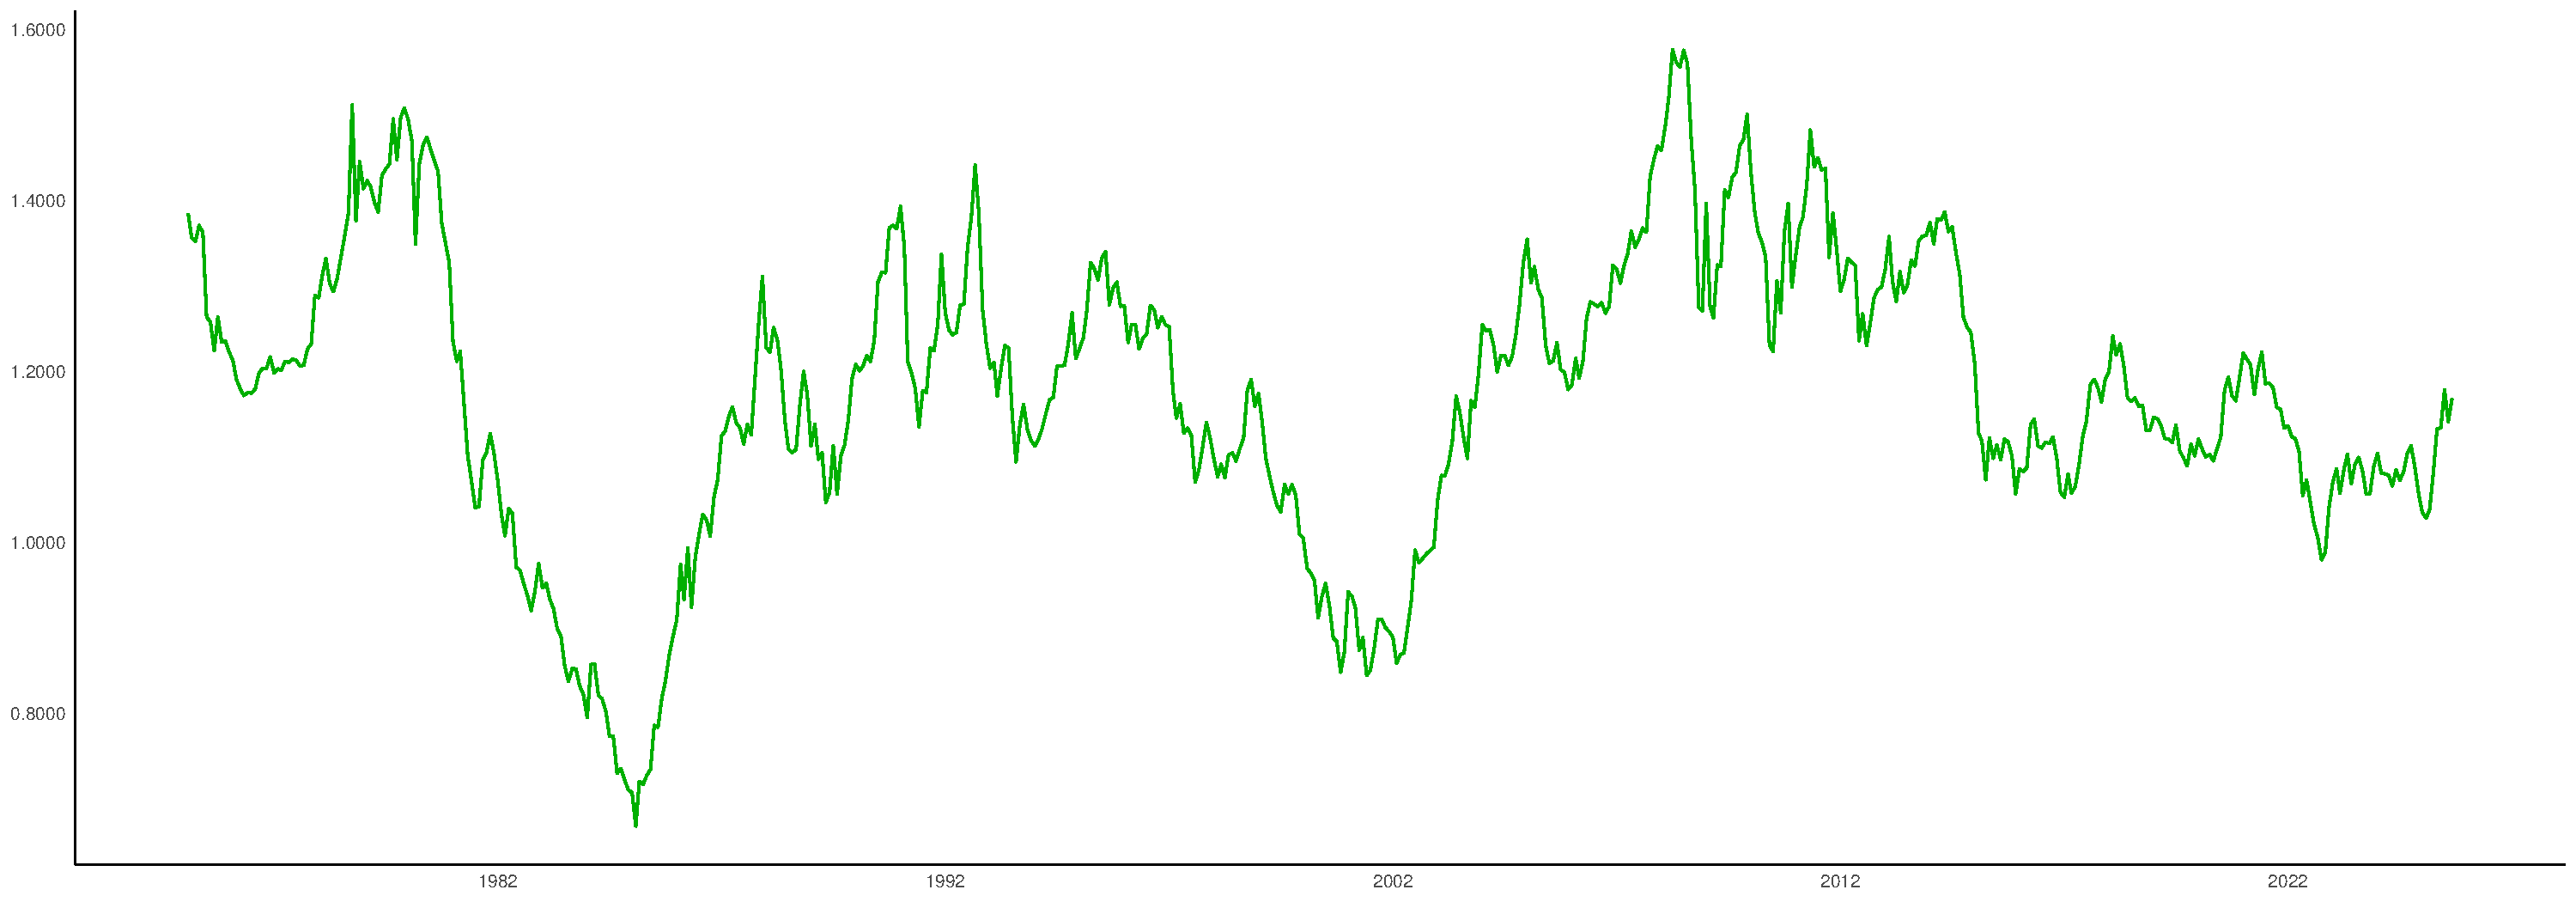
\includegraphics{Problemas_Propuestos_Regresion_Multinomial_files/figure-latex/unnamed-chunk-1-1.pdf}

\begin{Shaded}
\begin{Highlighting}[]
\FunctionTok{plot}\NormalTok{(iris)}
\end{Highlighting}
\end{Shaded}

\includegraphics{Problemas_Propuestos_Regresion_Multinomial_files/figure-latex/unnamed-chunk-1-2.pdf}

\begin{enumerate}
\def\labelenumi{\arabic{enumi})}
\setcounter{enumi}{1}
\tightlist
\item
  Dividir el conjunto de datos en entrenamiento y prueba (70\%
  entrenamiento, 30\% prueba). Tomar semilla 123.
\end{enumerate}

\begin{Shaded}
\begin{Highlighting}[]
\FunctionTok{set.seed}\NormalTok{(}\DecValTok{123}\NormalTok{)}

\NormalTok{split }\OtherTok{\textless{}{-}} \FunctionTok{sample}\NormalTok{(}\DecValTok{1}\SpecialCharTok{:}\FunctionTok{nrow}\NormalTok{(iris), }\FloatTok{0.7} \SpecialCharTok{*} \FunctionTok{nrow}\NormalTok{(iris))}

\CommentTok{\# Conjunto de entrenamiento}
\NormalTok{train\_data }\OtherTok{\textless{}{-}}\NormalTok{ iris[split, ]}

\CommentTok{\# Conjunto de prueba}
\NormalTok{test\_data }\OtherTok{\textless{}{-}}\NormalTok{ iris[}\SpecialCharTok{{-}}\NormalTok{split, ]}
\end{Highlighting}
\end{Shaded}

\begin{enumerate}
\def\labelenumi{\arabic{enumi})}
\setcounter{enumi}{2}
\tightlist
\item
  Con los datos de entrenamiento, obtener el modelo ajustado de
  Regresión Multinomial usando todos los predictores.
\end{enumerate}

\begin{Shaded}
\begin{Highlighting}[]
\FunctionTok{library}\NormalTok{(nnet)}
\NormalTok{iris}\SpecialCharTok{$}\NormalTok{Species }\OtherTok{\textless{}{-}} \FunctionTok{relevel}\NormalTok{(iris}\SpecialCharTok{$}\NormalTok{Species, }\AttributeTok{ref =} \StringTok{"setosa"}\NormalTok{)}
\NormalTok{modelo\_ajustado }\OtherTok{\textless{}{-}} \FunctionTok{multinom}\NormalTok{(Species }\SpecialCharTok{\textasciitilde{}}\NormalTok{ ., }\AttributeTok{data =}\NormalTok{ train\_data)}
\end{Highlighting}
\end{Shaded}

\begin{verbatim}
## # weights:  18 (10 variable)
## initial  value 115.354290 
## iter  10 value 14.037979
## iter  20 value 3.342288
## iter  30 value 2.503699
## iter  40 value 2.171547
## iter  50 value 2.099460
## iter  60 value 1.828506
## iter  70 value 0.904367
## iter  80 value 0.669147
## iter  90 value 0.622003
## iter 100 value 0.609416
## final  value 0.609416 
## stopped after 100 iterations
\end{verbatim}

\begin{Shaded}
\begin{Highlighting}[]
\FunctionTok{summary}\NormalTok{(modelo\_ajustado)}
\end{Highlighting}
\end{Shaded}

\begin{verbatim}
## Call:
## multinom(formula = Species ~ ., data = train_data)
## 
## Coefficients:
##            (Intercept) Sepal.Length Sepal.Width Petal.Length Petal.Width
## versicolor     63.7972    -27.80712   -27.99961      71.5816    18.78823
## virginica    -107.2881    -56.45906   -61.59348     140.6447    82.34126
## 
## Std. Errors:
##            (Intercept) Sepal.Length Sepal.Width Petal.Length Petal.Width
## versicolor    119.5758     41.53559    29.48294     45.30698    30.24145
## virginica     119.5759     41.53544    29.48285     45.30703    30.24145
## 
## Residual Deviance: 1.218832 
## AIC: 21.21883
\end{verbatim}

\begin{enumerate}
\def\labelenumi{\arabic{enumi})}
\setcounter{enumi}{3}
\tightlist
\item
  Con los datos de entrenamiento, aplicar los métodos de selección de
  regresores para comprobar si el modelo completo es reducible.
\end{enumerate}

\begin{Shaded}
\begin{Highlighting}[]
\NormalTok{modelo\_nulo }\OtherTok{\textless{}{-}} \FunctionTok{multinom}\NormalTok{(Species }\SpecialCharTok{\textasciitilde{}} \DecValTok{1}\NormalTok{, }\AttributeTok{data =}\NormalTok{ train\_data)}
\end{Highlighting}
\end{Shaded}

\begin{verbatim}
## # weights:  6 (2 variable)
## initial  value 115.354290 
## final  value 115.151643 
## converged
\end{verbatim}

\begin{Shaded}
\begin{Highlighting}[]
\NormalTok{modelo\_backward }\OtherTok{\textless{}{-}} \FunctionTok{step}\NormalTok{(modelo\_ajustado, }\AttributeTok{direction =} \StringTok{"backward"}\NormalTok{)}
\end{Highlighting}
\end{Shaded}

\begin{verbatim}
## Start:  AIC=21.22
## Species ~ Sepal.Length + Sepal.Width + Petal.Length + Petal.Width
## 
## trying - Sepal.Length 
## # weights:  15 (8 variable)
## initial  value 115.354290 
## iter  10 value 12.178204
## iter  20 value 5.050112
## iter  30 value 4.842539
## iter  40 value 4.731343
## iter  50 value 4.610612
## iter  60 value 4.597635
## final  value 4.596501 
## converged
## trying - Sepal.Width 
## # weights:  15 (8 variable)
## initial  value 115.354290 
## iter  10 value 9.870302
## iter  20 value 4.460007
## iter  30 value 4.407318
## iter  40 value 4.406430
## iter  50 value 4.403603
## iter  60 value 4.400206
## iter  70 value 4.398808
## iter  80 value 4.398415
## iter  90 value 4.398384
## iter 100 value 4.398316
## final  value 4.398316 
## stopped after 100 iterations
## trying - Petal.Length 
## # weights:  15 (8 variable)
## initial  value 115.354290 
## iter  10 value 13.208650
## iter  20 value 9.268575
## iter  30 value 8.984624
## iter  40 value 8.955823
## iter  50 value 8.953394
## final  value 8.953389 
## converged
## trying - Petal.Width 
## # weights:  15 (8 variable)
## initial  value 115.354290 
## iter  10 value 17.073901
## iter  20 value 7.858714
## iter  30 value 6.707280
## iter  40 value 6.406272
## iter  50 value 6.381857
## iter  60 value 6.374101
## final  value 6.366160 
## converged
##                Df      AIC
## <none>         10 21.21883
## - Sepal.Width   8 24.79663
## - Sepal.Length  8 25.19300
## - Petal.Width   8 28.73232
## - Petal.Length  8 33.90678
\end{verbatim}

\begin{Shaded}
\begin{Highlighting}[]
\NormalTok{modelo\_forward }\OtherTok{\textless{}{-}} \FunctionTok{step}\NormalTok{(modelo\_nulo, }\AttributeTok{direction =} \StringTok{"forward"}\NormalTok{, }\AttributeTok{scope =} \FunctionTok{formula}\NormalTok{(modelo\_ajustado))}
\end{Highlighting}
\end{Shaded}

\begin{verbatim}
## Start:  AIC=234.3
## Species ~ 1
## 
## trying + Sepal.Length 
## # weights:  9 (4 variable)
## initial  value 115.354290 
## iter  10 value 62.562717
## iter  20 value 62.200884
## iter  30 value 62.192424
## final  value 62.192209 
## converged
## trying + Sepal.Width 
## # weights:  9 (4 variable)
## initial  value 115.354290 
## iter  10 value 93.617609
## final  value 93.616396 
## converged
## trying + Petal.Length 
## # weights:  9 (4 variable)
## initial  value 115.354290 
## iter  10 value 14.092776
## iter  20 value 13.263608
## iter  30 value 13.152415
## iter  40 value 13.146931
## iter  50 value 13.146595
## iter  60 value 13.146399
## final  value 13.146285 
## converged
## trying + Petal.Width 
## # weights:  9 (4 variable)
## initial  value 115.354290 
## iter  10 value 13.287178
## iter  20 value 12.062553
## iter  30 value 11.998988
## iter  40 value 11.953176
## iter  50 value 11.950654
## iter  60 value 11.947170
## iter  70 value 11.946489
## iter  80 value 11.944525
## iter  90 value 11.944244
## iter 100 value 11.943668
## final  value 11.943668 
## stopped after 100 iterations
##                 Df       AIC
## + +Petal.Width   4  31.88734
## + +Petal.Length  4  34.29257
## + +Sepal.Length  4 132.38442
## + +Sepal.Width   4 195.23279
## <none>           2 234.30329
## # weights:  9 (4 variable)
## initial  value 115.354290 
## iter  10 value 13.287178
## iter  20 value 12.062553
## iter  30 value 11.998988
## iter  40 value 11.953176
## iter  50 value 11.950654
## iter  60 value 11.947170
## iter  70 value 11.946489
## iter  80 value 11.944525
## iter  90 value 11.944244
## iter 100 value 11.943668
## final  value 11.943668 
## stopped after 100 iterations
## 
## Step:  AIC=31.89
## Species ~ Petal.Width
## 
## trying + Sepal.Length 
## # weights:  12 (6 variable)
## initial  value 115.354290 
## iter  10 value 16.352816
## iter  20 value 12.454171
## iter  30 value 12.148159
## iter  40 value 11.905495
## iter  50 value 11.876547
## iter  60 value 11.875129
## iter  70 value 11.869701
## final  value 11.868493 
## converged
## trying + Sepal.Width 
## # weights:  12 (6 variable)
## initial  value 115.354290 
## iter  10 value 11.080002
## iter  20 value 9.789672
## iter  30 value 9.730231
## iter  40 value 9.691618
## iter  50 value 9.679265
## iter  60 value 9.670540
## iter  70 value 9.668341
## iter  80 value 9.660126
## iter  90 value 9.658204
## iter 100 value 9.658102
## final  value 9.658102 
## stopped after 100 iterations
## trying + Petal.Length 
## # weights:  12 (6 variable)
## initial  value 115.354290 
## iter  10 value 10.604971
## iter  20 value 8.547740
## iter  30 value 8.513403
## iter  40 value 8.500973
## iter  50 value 8.494082
## iter  60 value 8.492201
## iter  70 value 8.487866
## iter  80 value 8.486032
## iter  90 value 8.484822
## iter 100 value 8.483691
## final  value 8.483691 
## stopped after 100 iterations
##                 Df      AIC
## + +Petal.Length  6 28.96738
## + +Sepal.Width   6 31.31620
## <none>           4 31.88734
## + +Sepal.Length  6 35.73699
## # weights:  12 (6 variable)
## initial  value 115.354290 
## iter  10 value 10.604971
## iter  20 value 8.547740
## iter  30 value 8.513403
## iter  40 value 8.500973
## iter  50 value 8.494082
## iter  60 value 8.492201
## iter  70 value 8.487866
## iter  80 value 8.486032
## iter  90 value 8.484822
## iter 100 value 8.483691
## final  value 8.483691 
## stopped after 100 iterations
## 
## Step:  AIC=28.97
## Species ~ Petal.Width + Petal.Length
## 
## trying + Sepal.Length 
## # weights:  15 (8 variable)
## initial  value 115.354290 
## iter  10 value 9.870302
## iter  20 value 4.460007
## iter  30 value 4.407318
## iter  40 value 4.406430
## iter  50 value 4.403603
## iter  60 value 4.400206
## iter  70 value 4.398808
## iter  80 value 4.398415
## iter  90 value 4.398384
## iter 100 value 4.398316
## final  value 4.398316 
## stopped after 100 iterations
## trying + Sepal.Width 
## # weights:  15 (8 variable)
## initial  value 115.354290 
## iter  10 value 12.178204
## iter  20 value 5.050112
## iter  30 value 4.842539
## iter  40 value 4.731343
## iter  50 value 4.610612
## iter  60 value 4.597635
## final  value 4.596501 
## converged
##                 Df      AIC
## + +Sepal.Length  8 24.79663
## + +Sepal.Width   8 25.19300
## <none>           6 28.96738
## # weights:  15 (8 variable)
## initial  value 115.354290 
## iter  10 value 9.870302
## iter  20 value 4.460007
## iter  30 value 4.407318
## iter  40 value 4.406430
## iter  50 value 4.403603
## iter  60 value 4.400206
## iter  70 value 4.398808
## iter  80 value 4.398415
## iter  90 value 4.398384
## iter 100 value 4.398316
## final  value 4.398316 
## stopped after 100 iterations
## 
## Step:  AIC=24.8
## Species ~ Petal.Width + Petal.Length + Sepal.Length
## 
## trying + Sepal.Width 
## # weights:  18 (10 variable)
## initial  value 115.354290 
## iter  10 value 14.037979
## iter  20 value 3.342288
## iter  30 value 2.503699
## iter  40 value 2.171547
## iter  50 value 2.099460
## iter  60 value 1.828506
## iter  70 value 0.904367
## iter  80 value 0.669147
## iter  90 value 0.622003
## iter 100 value 0.609416
## final  value 0.609416 
## stopped after 100 iterations
##                Df      AIC
## + +Sepal.Width 10 21.21883
## <none>          8 24.79663
## # weights:  18 (10 variable)
## initial  value 115.354290 
## iter  10 value 14.037979
## iter  20 value 3.342288
## iter  30 value 2.503699
## iter  40 value 2.171547
## iter  50 value 2.099460
## iter  60 value 1.828506
## iter  70 value 0.904367
## iter  80 value 0.669147
## iter  90 value 0.622003
## iter 100 value 0.609416
## final  value 0.609416 
## stopped after 100 iterations
## 
## Step:  AIC=21.22
## Species ~ Petal.Width + Petal.Length + Sepal.Length + Sepal.Width
\end{verbatim}

\begin{Shaded}
\begin{Highlighting}[]
\NormalTok{modelo\_stepwise }\OtherTok{\textless{}{-}} \FunctionTok{step}\NormalTok{(modelo\_nulo, }\AttributeTok{direction =} \StringTok{"both"}\NormalTok{, }\AttributeTok{scope =} \FunctionTok{formula}\NormalTok{(modelo\_ajustado))}
\end{Highlighting}
\end{Shaded}

\begin{verbatim}
## Start:  AIC=234.3
## Species ~ 1
## 
## trying + Sepal.Length 
## # weights:  9 (4 variable)
## initial  value 115.354290 
## iter  10 value 62.562717
## iter  20 value 62.200884
## iter  30 value 62.192424
## final  value 62.192209 
## converged
## trying + Sepal.Width 
## # weights:  9 (4 variable)
## initial  value 115.354290 
## iter  10 value 93.617609
## final  value 93.616396 
## converged
## trying + Petal.Length 
## # weights:  9 (4 variable)
## initial  value 115.354290 
## iter  10 value 14.092776
## iter  20 value 13.263608
## iter  30 value 13.152415
## iter  40 value 13.146931
## iter  50 value 13.146595
## iter  60 value 13.146399
## final  value 13.146285 
## converged
## trying + Petal.Width 
## # weights:  9 (4 variable)
## initial  value 115.354290 
## iter  10 value 13.287178
## iter  20 value 12.062553
## iter  30 value 11.998988
## iter  40 value 11.953176
## iter  50 value 11.950654
## iter  60 value 11.947170
## iter  70 value 11.946489
## iter  80 value 11.944525
## iter  90 value 11.944244
## iter 100 value 11.943668
## final  value 11.943668 
## stopped after 100 iterations
##                 Df       AIC
## + +Petal.Width   4  31.88734
## + +Petal.Length  4  34.29257
## + +Sepal.Length  4 132.38442
## + +Sepal.Width   4 195.23279
## <none>           2 234.30329
## # weights:  9 (4 variable)
## initial  value 115.354290 
## iter  10 value 13.287178
## iter  20 value 12.062553
## iter  30 value 11.998988
## iter  40 value 11.953176
## iter  50 value 11.950654
## iter  60 value 11.947170
## iter  70 value 11.946489
## iter  80 value 11.944525
## iter  90 value 11.944244
## iter 100 value 11.943668
## final  value 11.943668 
## stopped after 100 iterations
## 
## Step:  AIC=31.89
## Species ~ Petal.Width
## 
## trying - Petal.Width 
## # weights:  6 (2 variable)
## initial  value 115.354290 
## final  value 115.151643 
## converged
## trying + Sepal.Length 
## # weights:  12 (6 variable)
## initial  value 115.354290 
## iter  10 value 16.352816
## iter  20 value 12.454171
## iter  30 value 12.148159
## iter  40 value 11.905495
## iter  50 value 11.876547
## iter  60 value 11.875129
## iter  70 value 11.869701
## final  value 11.868493 
## converged
## trying + Sepal.Width 
## # weights:  12 (6 variable)
## initial  value 115.354290 
## iter  10 value 11.080002
## iter  20 value 9.789672
## iter  30 value 9.730231
## iter  40 value 9.691618
## iter  50 value 9.679265
## iter  60 value 9.670540
## iter  70 value 9.668341
## iter  80 value 9.660126
## iter  90 value 9.658204
## iter 100 value 9.658102
## final  value 9.658102 
## stopped after 100 iterations
## trying + Petal.Length 
## # weights:  12 (6 variable)
## initial  value 115.354290 
## iter  10 value 10.604971
## iter  20 value 8.547740
## iter  30 value 8.513403
## iter  40 value 8.500973
## iter  50 value 8.494082
## iter  60 value 8.492201
## iter  70 value 8.487866
## iter  80 value 8.486032
## iter  90 value 8.484822
## iter 100 value 8.483691
## final  value 8.483691 
## stopped after 100 iterations
##                 Df       AIC
## + +Petal.Length  6  28.96738
## + +Sepal.Width   6  31.31620
## <none>           4  31.88734
## + +Sepal.Length  6  35.73699
## - Petal.Width    2 234.30329
## # weights:  12 (6 variable)
## initial  value 115.354290 
## iter  10 value 10.604971
## iter  20 value 8.547740
## iter  30 value 8.513403
## iter  40 value 8.500973
## iter  50 value 8.494082
## iter  60 value 8.492201
## iter  70 value 8.487866
## iter  80 value 8.486032
## iter  90 value 8.484822
## iter 100 value 8.483691
## final  value 8.483691 
## stopped after 100 iterations
## 
## Step:  AIC=28.97
## Species ~ Petal.Width + Petal.Length
## 
## trying - Petal.Width 
## # weights:  9 (4 variable)
## initial  value 115.354290 
## iter  10 value 14.092776
## iter  20 value 13.263608
## iter  30 value 13.152415
## iter  40 value 13.146931
## iter  50 value 13.146595
## iter  60 value 13.146399
## final  value 13.146285 
## converged
## trying - Petal.Length 
## # weights:  9 (4 variable)
## initial  value 115.354290 
## iter  10 value 13.287178
## iter  20 value 12.062553
## iter  30 value 11.998988
## iter  40 value 11.953176
## iter  50 value 11.950654
## iter  60 value 11.947170
## iter  70 value 11.946489
## iter  80 value 11.944525
## iter  90 value 11.944244
## iter 100 value 11.943668
## final  value 11.943668 
## stopped after 100 iterations
## trying + Sepal.Length 
## # weights:  15 (8 variable)
## initial  value 115.354290 
## iter  10 value 9.870302
## iter  20 value 4.460007
## iter  30 value 4.407318
## iter  40 value 4.406430
## iter  50 value 4.403603
## iter  60 value 4.400206
## iter  70 value 4.398808
## iter  80 value 4.398415
## iter  90 value 4.398384
## iter 100 value 4.398316
## final  value 4.398316 
## stopped after 100 iterations
## trying + Sepal.Width 
## # weights:  15 (8 variable)
## initial  value 115.354290 
## iter  10 value 12.178204
## iter  20 value 5.050112
## iter  30 value 4.842539
## iter  40 value 4.731343
## iter  50 value 4.610612
## iter  60 value 4.597635
## final  value 4.596501 
## converged
##                 Df      AIC
## + +Sepal.Length  8 24.79663
## + +Sepal.Width   8 25.19300
## <none>           6 28.96738
## - Petal.Length   4 31.88734
## - Petal.Width    4 34.29257
## # weights:  15 (8 variable)
## initial  value 115.354290 
## iter  10 value 9.870302
## iter  20 value 4.460007
## iter  30 value 4.407318
## iter  40 value 4.406430
## iter  50 value 4.403603
## iter  60 value 4.400206
## iter  70 value 4.398808
## iter  80 value 4.398415
## iter  90 value 4.398384
## iter 100 value 4.398316
## final  value 4.398316 
## stopped after 100 iterations
## 
## Step:  AIC=24.8
## Species ~ Petal.Width + Petal.Length + Sepal.Length
## 
## trying - Petal.Width 
## # weights:  12 (6 variable)
## initial  value 115.354290 
## iter  10 value 12.488824
## iter  20 value 6.973806
## iter  30 value 6.639299
## iter  40 value 6.563502
## iter  50 value 6.508959
## iter  60 value 6.488786
## iter  70 value 6.487951
## iter  80 value 6.486000
## iter  90 value 6.485869
## iter 100 value 6.485675
## final  value 6.485675 
## stopped after 100 iterations
## trying - Petal.Length 
## # weights:  12 (6 variable)
## initial  value 115.354290 
## iter  10 value 16.352816
## iter  20 value 12.454171
## iter  30 value 12.148159
## iter  40 value 11.905495
## iter  50 value 11.876547
## iter  60 value 11.875129
## iter  70 value 11.869701
## final  value 11.868493 
## converged
## trying - Sepal.Length 
## # weights:  12 (6 variable)
## initial  value 115.354290 
## iter  10 value 10.604971
## iter  20 value 8.547740
## iter  30 value 8.513403
## iter  40 value 8.500973
## iter  50 value 8.494082
## iter  60 value 8.492201
## iter  70 value 8.487866
## iter  80 value 8.486032
## iter  90 value 8.484822
## iter 100 value 8.483691
## final  value 8.483691 
## stopped after 100 iterations
## trying + Sepal.Width 
## # weights:  18 (10 variable)
## initial  value 115.354290 
## iter  10 value 14.037979
## iter  20 value 3.342288
## iter  30 value 2.503699
## iter  40 value 2.171547
## iter  50 value 2.099460
## iter  60 value 1.828506
## iter  70 value 0.904367
## iter  80 value 0.669147
## iter  90 value 0.622003
## iter 100 value 0.609416
## final  value 0.609416 
## stopped after 100 iterations
##                Df      AIC
## + +Sepal.Width 10 21.21883
## <none>          8 24.79663
## - Petal.Width   6 24.97135
## - Sepal.Length  6 28.96738
## - Petal.Length  6 35.73699
## # weights:  18 (10 variable)
## initial  value 115.354290 
## iter  10 value 14.037979
## iter  20 value 3.342288
## iter  30 value 2.503699
## iter  40 value 2.171547
## iter  50 value 2.099460
## iter  60 value 1.828506
## iter  70 value 0.904367
## iter  80 value 0.669147
## iter  90 value 0.622003
## iter 100 value 0.609416
## final  value 0.609416 
## stopped after 100 iterations
## 
## Step:  AIC=21.22
## Species ~ Petal.Width + Petal.Length + Sepal.Length + Sepal.Width
## 
## trying - Petal.Width 
## # weights:  15 (8 variable)
## initial  value 115.354290 
## iter  10 value 17.073901
## iter  20 value 7.858714
## iter  30 value 6.707280
## iter  40 value 6.406272
## iter  50 value 6.381857
## iter  60 value 6.374101
## final  value 6.366160 
## converged
## trying - Petal.Length 
## # weights:  15 (8 variable)
## initial  value 115.354290 
## iter  10 value 13.208650
## iter  20 value 9.268575
## iter  30 value 8.984624
## iter  40 value 8.955823
## iter  50 value 8.953394
## final  value 8.953389 
## converged
## trying - Sepal.Length 
## # weights:  15 (8 variable)
## initial  value 115.354290 
## iter  10 value 12.178204
## iter  20 value 5.050112
## iter  30 value 4.842539
## iter  40 value 4.731343
## iter  50 value 4.610612
## iter  60 value 4.597635
## final  value 4.596501 
## converged
## trying - Sepal.Width 
## # weights:  15 (8 variable)
## initial  value 115.354290 
## iter  10 value 9.870302
## iter  20 value 4.460007
## iter  30 value 4.407318
## iter  40 value 4.406430
## iter  50 value 4.403603
## iter  60 value 4.400206
## iter  70 value 4.398808
## iter  80 value 4.398415
## iter  90 value 4.398384
## iter 100 value 4.398316
## final  value 4.398316 
## stopped after 100 iterations
##                Df      AIC
## <none>         10 21.21883
## - Sepal.Width   8 24.79663
## - Sepal.Length  8 25.19300
## - Petal.Width   8 28.73232
## - Petal.Length  8 33.90678
\end{verbatim}

\begin{enumerate}
\def\labelenumi{\arabic{enumi})}
\setcounter{enumi}{4}
\tightlist
\item
  Con el modelo resultante del apartado anterior, obtener medidas de
  bondad del ajuste e indicar si el modelo es significativo.
\end{enumerate}

\begin{Shaded}
\begin{Highlighting}[]
\CommentTok{\# Bondad del ajuste}
\FunctionTok{paste}\NormalTok{(}\StringTok{"Bondad del ajuste ="}\NormalTok{, modelo\_ajustado}\SpecialCharTok{$}\NormalTok{AIC)}
\end{Highlighting}
\end{Shaded}

\begin{verbatim}
## [1] "Bondad del ajuste = 21.2188317697612"
\end{verbatim}

\begin{Shaded}
\begin{Highlighting}[]
\CommentTok{\# Significación del modelo}
\NormalTok{diferencia\_desvianza }\OtherTok{\textless{}{-}}\NormalTok{ modelo\_nulo}\SpecialCharTok{$}\NormalTok{deviance }\SpecialCharTok{{-}}\NormalTok{ modelo\_ajustado}\SpecialCharTok{$}\NormalTok{deviance}

\NormalTok{df\_nulo }\OtherTok{\textless{}{-}} \FunctionTok{length}\NormalTok{(iris}\SpecialCharTok{$}\NormalTok{Species) }\SpecialCharTok{{-}} \DecValTok{1}
\NormalTok{df\_ajustado }\OtherTok{\textless{}{-}} \FunctionTok{length}\NormalTok{(iris}\SpecialCharTok{$}\NormalTok{Species) }\SpecialCharTok{{-}} \FunctionTok{length}\NormalTok{(modelo\_ajustado}\SpecialCharTok{$}\NormalTok{coefnames) }\SpecialCharTok{{-}} \DecValTok{1}

\NormalTok{grados\_libertad }\OtherTok{\textless{}{-}}\NormalTok{ df\_nulo }\SpecialCharTok{{-}}\NormalTok{ df\_ajustado}

\NormalTok{p\_valor }\OtherTok{\textless{}{-}} \FunctionTok{pchisq}\NormalTok{(diferencia\_desvianza, }\AttributeTok{df =}\NormalTok{ grados\_libertad, }\AttributeTok{lower.tail =} \ConstantTok{FALSE}\NormalTok{)}

\NormalTok{p\_valor}
\end{Highlighting}
\end{Shaded}

\begin{verbatim}
## [1] 1.680466e-47
\end{verbatim}

El resultado de \texttt{p-valor} permite concluir que el modelo completo
es significativo

\begin{enumerate}
\def\labelenumi{\arabic{enumi})}
\setcounter{enumi}{5}
\tightlist
\item
  Veamos ahora el problema de Regresión Multinomial como un problema de
  clasificación. Obtener la clase predicha para los datos del conjunto
  de prueba.
\end{enumerate}

\begin{Shaded}
\begin{Highlighting}[]
\NormalTok{species\_predict }\OtherTok{\textless{}{-}} \FunctionTok{predict}\NormalTok{(modelo\_ajustado, }\AttributeTok{newdata =}\NormalTok{ iris, }\StringTok{"class"}\NormalTok{)}
\NormalTok{iris\_predict }\OtherTok{\textless{}{-}} \FunctionTok{cbind}\NormalTok{(iris, species\_predict)}
\end{Highlighting}
\end{Shaded}

\begin{enumerate}
\def\labelenumi{\arabic{enumi})}
\setcounter{enumi}{6}
\tightlist
\item
  Obtener la matriz de confusión para el conjunto de prueba y medir la
  eficiencia del clasificador con el ``accuracy'' (número de aciertos en
  la clasificación dividido entre número de datos totales).
\end{enumerate}

\begin{Shaded}
\begin{Highlighting}[]
\NormalTok{matriz\_confusion }\OtherTok{\textless{}{-}} \FunctionTok{table}\NormalTok{(iris\_predict}\SpecialCharTok{$}\NormalTok{Species, iris\_predict}\SpecialCharTok{$}\NormalTok{species\_predict,}
                          \AttributeTok{dnn =} \FunctionTok{c}\NormalTok{(}\StringTok{"real"}\NormalTok{, }\StringTok{"predicho"}\NormalTok{))}
\NormalTok{matriz\_confusion}
\end{Highlighting}
\end{Shaded}

\begin{verbatim}
##             predicho
## real         setosa versicolor virginica
##   setosa         50          0         0
##   versicolor      0         49         1
##   virginica       0          0        50
\end{verbatim}

\begin{Shaded}
\begin{Highlighting}[]
\NormalTok{accuracy }\OtherTok{\textless{}{-}} \FunctionTok{sum}\NormalTok{(}\FunctionTok{diag}\NormalTok{(matriz\_confusion)) }\SpecialCharTok{/} \FunctionTok{sum}\NormalTok{(matriz\_confusion)}
\NormalTok{accuracy}
\end{Highlighting}
\end{Shaded}

\begin{verbatim}
## [1] 0.9933333
\end{verbatim}

\end{document}
